\documentclass[notitlepage]{report}

\title{
	\textsc{ \small
		Physics 415
	} \\
	{\textsc{\small Lab \#5}} \\
	Two-Slit Interference, One Photon at a Time
}
\author{Kevin Evans \\ Partner: Sierra Ray}
\date{March 30, 2021}
\usepackage{amssymb}
\usepackage{mathtools}

\usepackage{amsthm}
\usepackage{amsmath}
\usepackage{slashed}
\usepackage{relsize}
\usepackage{threeparttable}
\usepackage{float}
\usepackage{booktabs}
\usepackage{boldline}
\usepackage{changepage}
\usepackage{physics}
\usepackage[inter-unit-product =\cdot]{siunitx}
\usepackage{setspace}
\usepackage{caption}
\usepackage{subcaption}
\usepackage[makeroom]{cancel}
%\usepackage{pgfplots}

\usepackage{enumitem}
\usepackage{times}
\usepackage{titling} % for titlingpage environment
\usepackage{calligra}
\usepackage{graphicx}
\DeclareMathAlphabet{\mathcalligra}{T1}{calligra}{m}{n}
\DeclareFontShape{T1}{calligra}{m}{n}{<->s*[2.2]callig15}{}
\newcommand{\scriptr}{\mathcalligra{r}\,}
\newcommand{\boldscriptr}{\pmb{\mathcalligra{r}}\,}
\newcommand{\emf}{\mathcal{E}}
\renewcommand{\thesection}{\arabic{section}}

\begin{document}
	\begin{titlingpage}
		\maketitle
		\begin{abstract}
			\noindent In this experiment, the wave-particle duality of photons was observed using two sources: a laser and an incandescent bulb. Light from each of these sources was passed through a single and double slit, resulting in an interference pattern. This data was plotted in Origin with a nonlinear curve fit applied. 
			For the laser, the average slit width was found to be \SI{44.65}{\um} $\pm$ \SI{1.55}{\um}. From the double slit, the slit distance was found to be \SI{178}{\um} $\pm$ \SI{0.321}{\um}. For the incandescent bulb, the slit width resulted in \SI{62.5}{\um} $\pm$ \SI{2.9}{\um}. The distance between the two slits was calculated to be \SI{354}{\um}.
		\end{abstract}
	\end{titlingpage}
	
	\section{Description of Experiment}
	In this experiment, the wave-particle duality of photons was observed. Initially, a monochromatic laser with wavelength \SI{670}{\nm} was used. A two slit blocker was placed in front of the laser with an adjustable translation stage placed in front, allowing four configurations: no light passing through, far slit blocked, near slit blocked, both slits open. The locations of each of these configurations was noted, allowing the configuration to be know when the cover of the apparatus was closed. A photodiode was connected to the voltmeter about \SI{50}{\centi\meter} from the slits. The voltages for each configuration was recorded. Then, for each configuration, a slit blocker was systematically adjusted between \SI{0}{\mm} to about \SI{10}{\mm} and the intensities relative to the translation distances was recorded in Origin.
	
	\subsubsection{Single-photon mode}
	The laser was switched off and an incadescent bulb was used as the light source instead. A filter was placed in front of the light to reduce the emitted power. Instead of the photodiode recording the intensities, a photomultiplier tube (PMT) was used. The PMT was initially set at a \SI{500}{\V} bias and the discriminator was set to setting 4. The output of the discriminator was attached to a frequency counter, which displayed the photon counts per second.
	
	\begin{figure}[H]
		\centering
		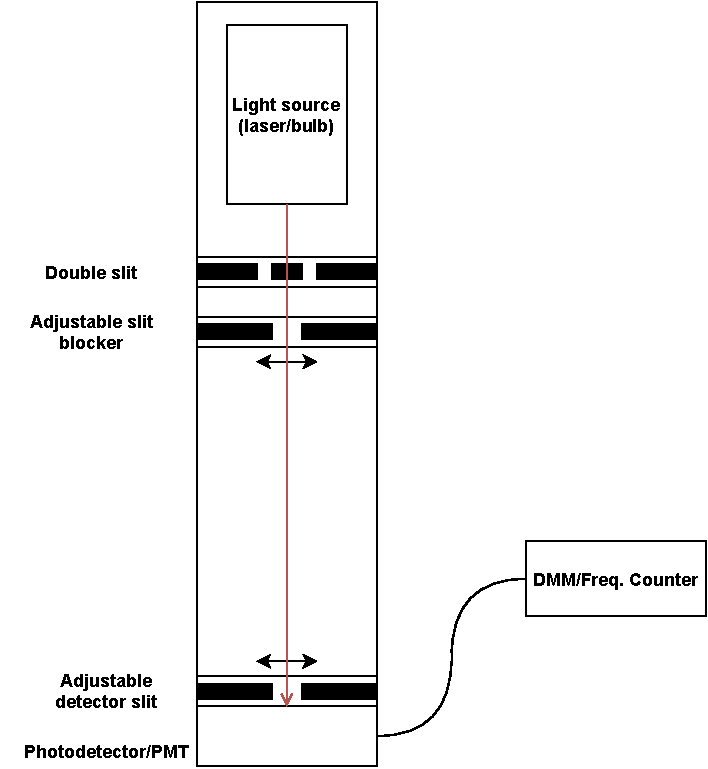
\includegraphics[width=0.5\linewidth]{setup}
		\caption{Diagram of the experimental setup (TeachSpin apparatus).}
		\label{fig:setup}
	\end{figure}
	
	\section{Data and Analysis}
	The slit blocker location of each configuration was recorded in Table \ref{table:translations}. For laser light, the slit blocker was adjusted and the relative intensities was recorded in Origin. This data was then plotted, shown in Figure \ref{fig:graph6} and \ref{fig:graph7}. From these three, the average slit width was found to be \SI{44.65}{\um} $\pm$ \SI{1.55}{\um}. From the double slit, the slit distance was found to be \SI{178}{\um} $\pm$ \SI{0.321}{\um}. 
	
	This is somewhat far from the expected value of width \SI{85}{\um} and \SI{353}{\um}. The expected values are roughly twice as large, which may mean there is a factor of $2$ missing in the curve fit. If doubled, the relative error for the slit width and distance is 5.1\% and 0.008\% respectively.
	
	In single-photon mode, the photon counts was recorded in Origin and plotted. This is shown in Figures \ref{fig:graph8} and \ref{fig:graph9}. These plots had relatively poor fits, possibly stemming from light leakage across the first blocker. The light is no longer coherent and has an additional envelope. 
	
	Averaging the slit width results in \SI{62.5}{\um} $\pm$ \SI{2.9}{\um}. The distance between the two slits was calculated to be \SI{354}{\um}. The relative error for the slit width and distance was found to be 26.4\% and 0.2\% respectively.
	
	At the maximum peak, the frequency counter read 29799 counts, leading to an average time of \SI{33.56}{\us} between successive photons. The transit time can be calculated from $t=d/c$, and for the half meter, the transit time is \SI{1.67}{\ns}.
		

	
	\begin{figure}[p]
		\centering
		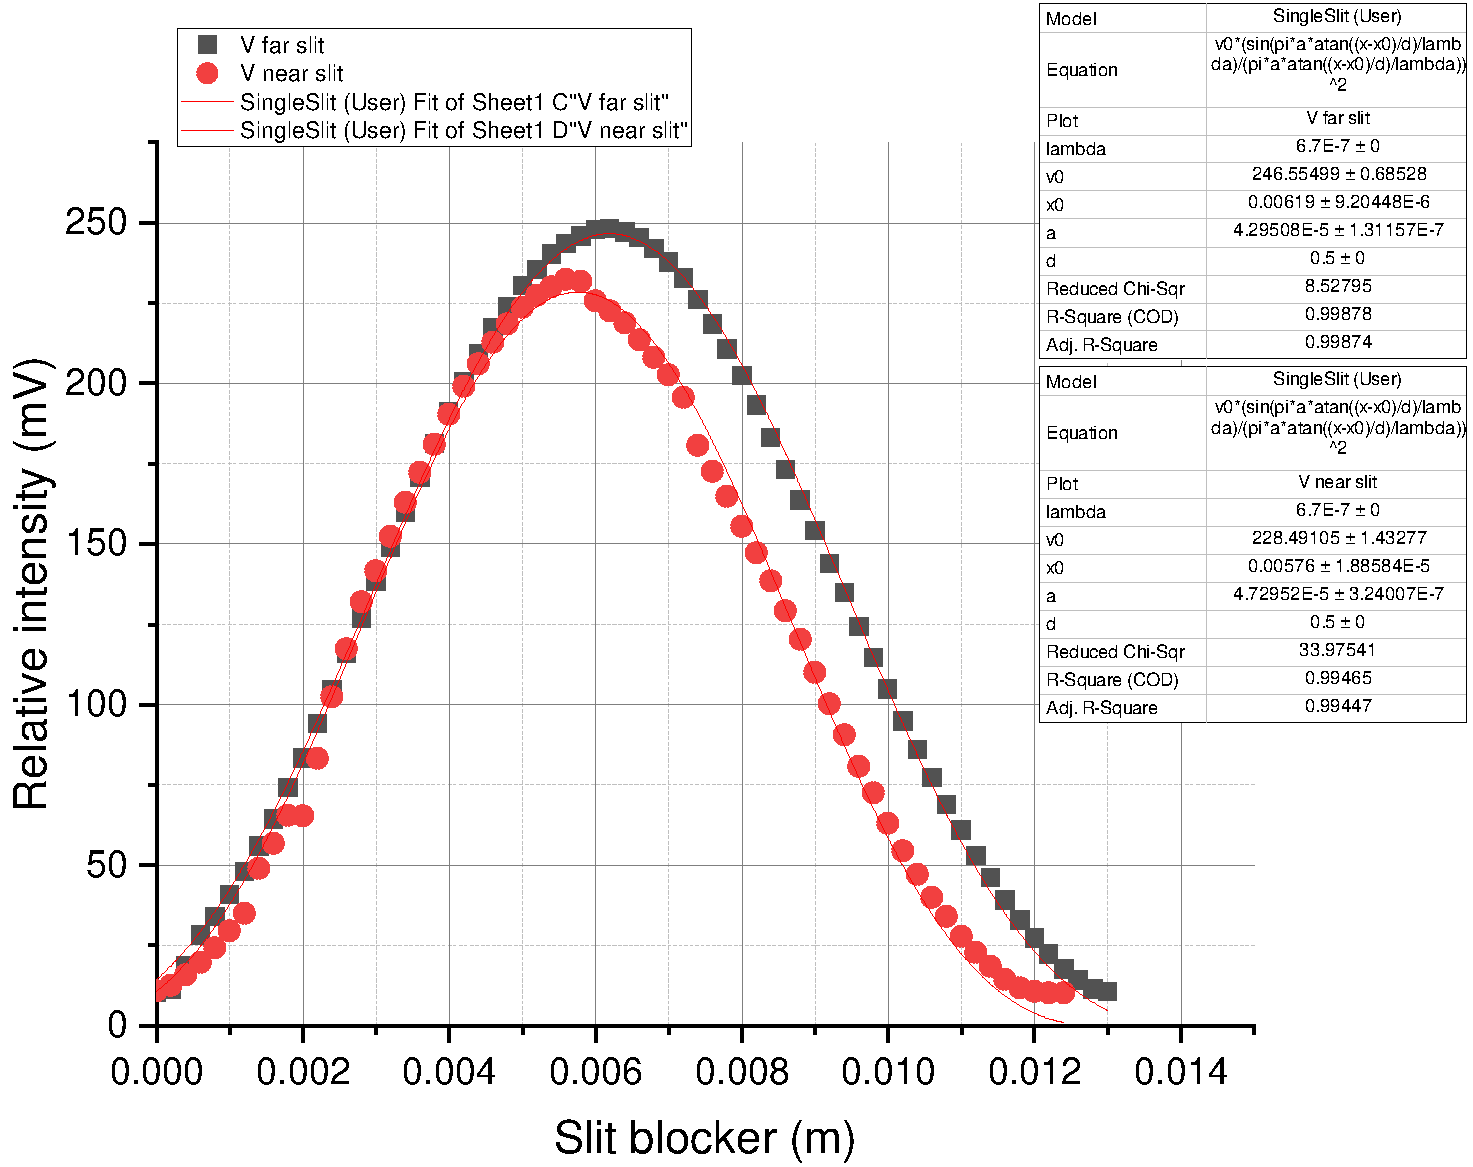
\includegraphics[width=0.7\linewidth]{Graph6}
		\caption{Relative intensities and curve fit of laser light passing through a single slit.}
		\label{fig:graph6}
	\end{figure}
	
	\begin{figure}[p]
		\centering
		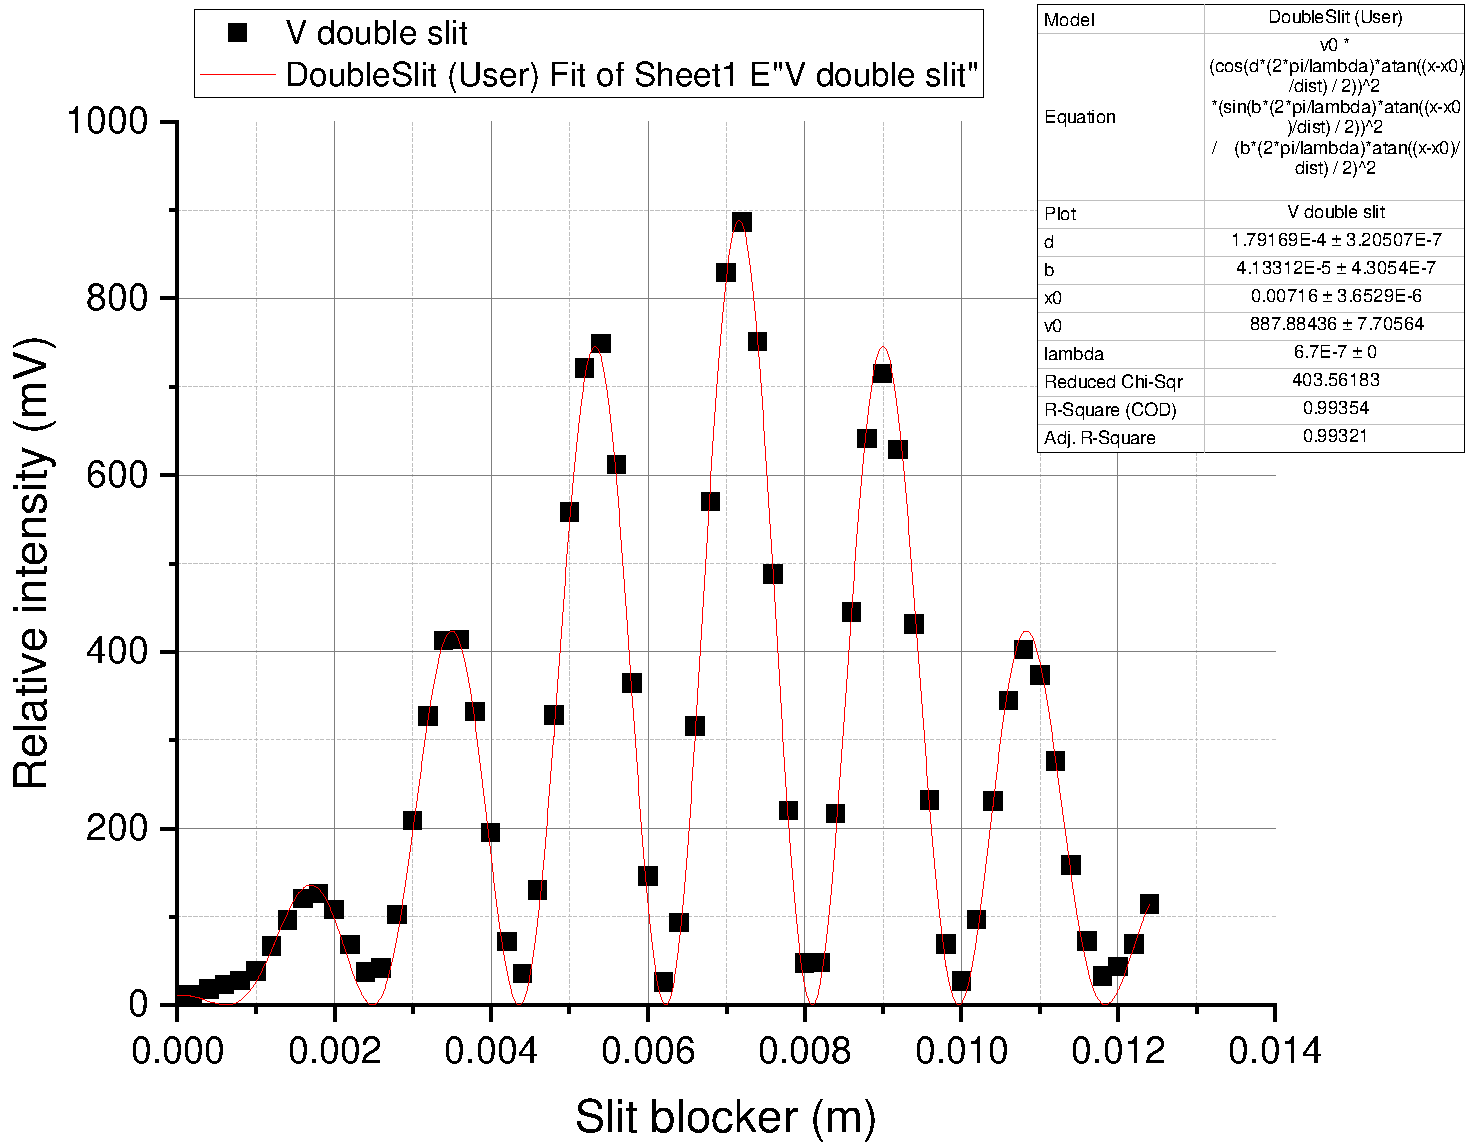
\includegraphics[width=0.7\linewidth]{Graph7}
		\caption{Relative intensities and curve fit of laser light passing through both slits.}
		\label{fig:graph7}
	\end{figure}
	

		
	\begin{figure}[p]
		\centering
		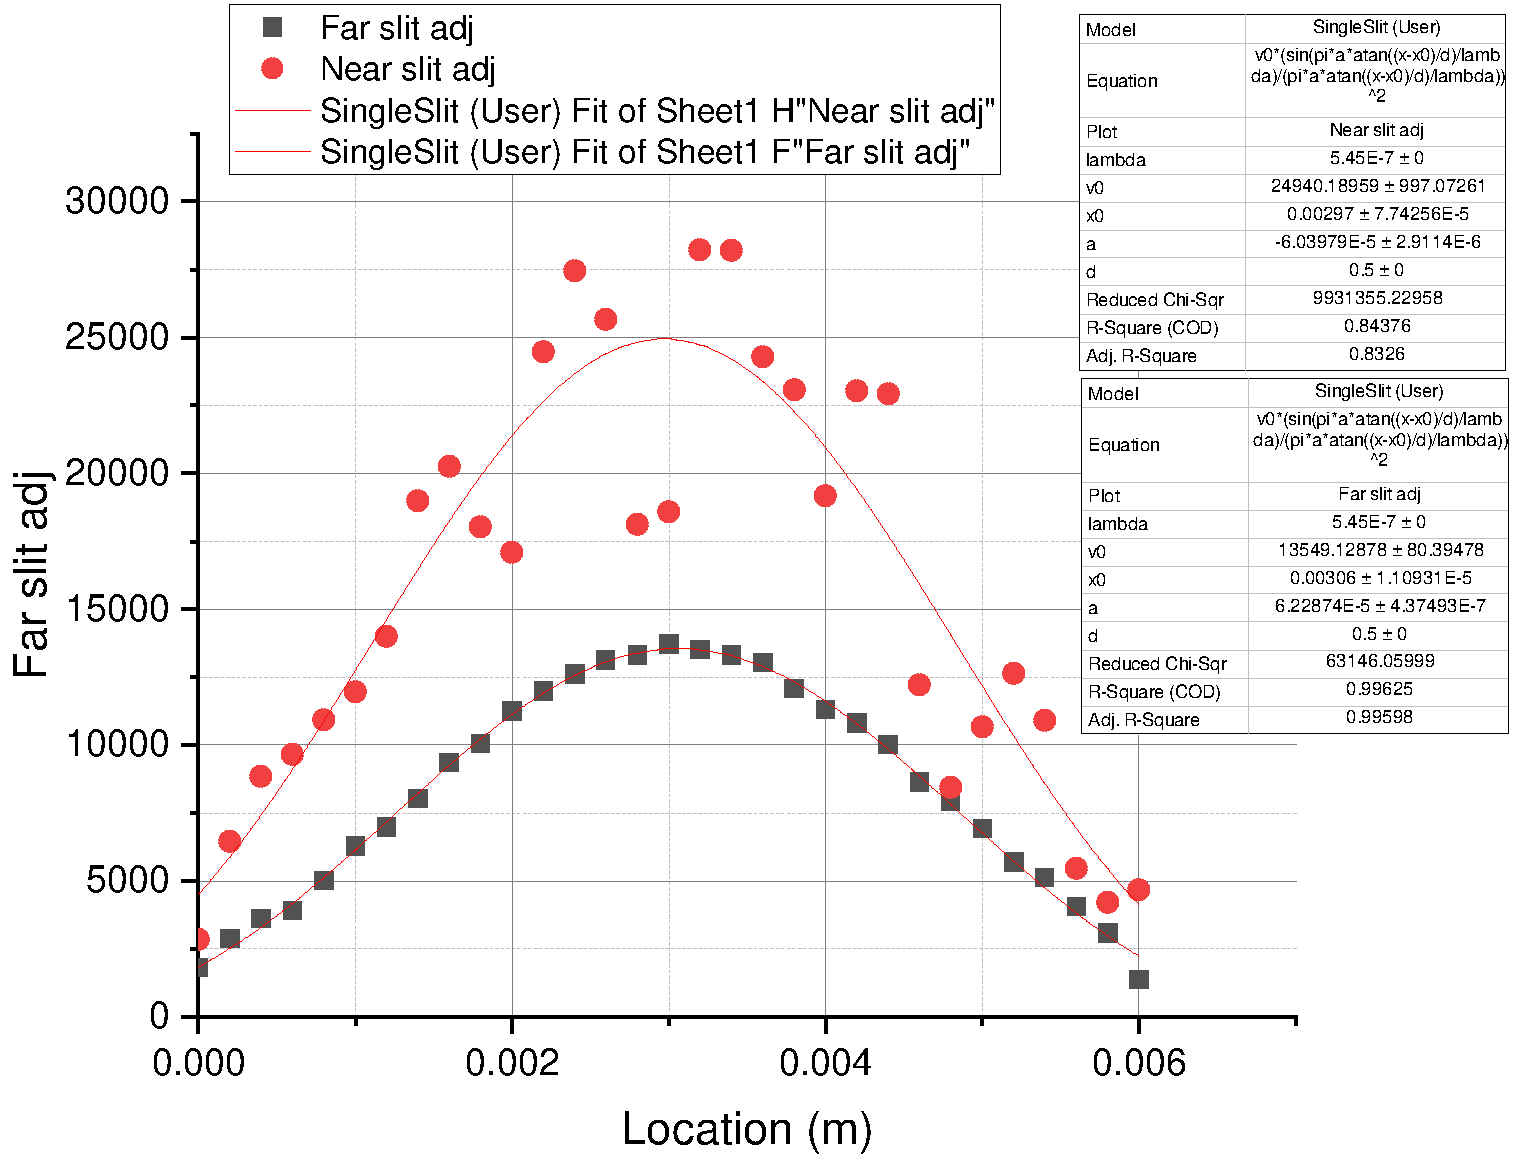
\includegraphics[width=0.7\linewidth]{Graph9}
		\caption{Single photon counts and curve fit of light passing through both slits.}
		\label{fig:graph9}
	\end{figure}
	\begin{figure}[p]
		\centering
		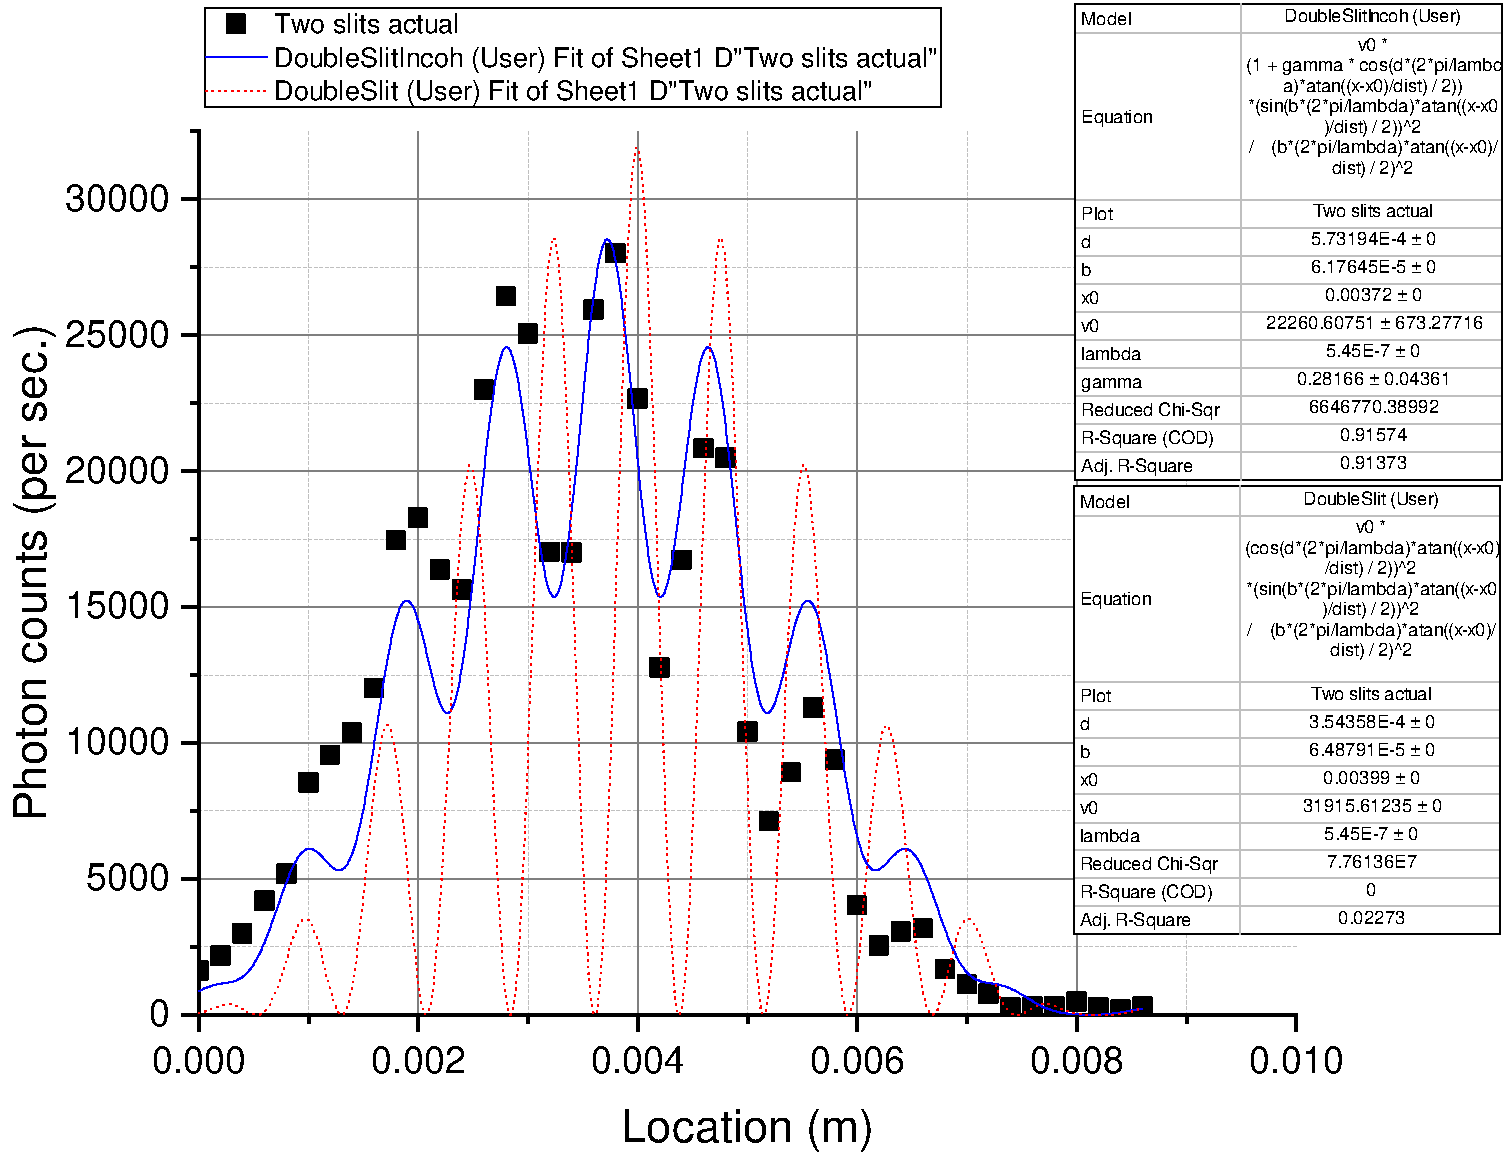
\includegraphics[width=0.7\linewidth]{Graph8}
		\caption{Single photon counts and curve fit of light passing through a single slit. Two fits are used here: the blue fit includes a term for incoherent light (due to error), whereas the red fit does not.}
		\label{fig:graph8}
	\end{figure}

	
	\section{Results and Conclusion}
	Despite the poor fit for several plots, the relative error for the slit distance was low, both at $<1\%$ for the laser and single photon beams. However, the relative error for the slit width was considerably higher at 5.1\% and 26.4\%. The poor fit and high error may have several causes. As discussed previously, there was likely light leakage past the first slit blocker resulting in incoherent light. In future iterations, it would be better to spend more time aligning the slit blocker and measuring the exact translation of each configuration.
	
	\pagebreak
	\section*{Data tables}
	\begin{table}[H]
		\centering
		\caption{Slit configurations and corresponding translation distances.}
		\label{table:translations}
		\begin{tabular}{ccc}
			\toprule
			Configuration & Translation (mm) & Observation \\
			\midrule
			Both slits blocked & $0.00$ & No light \\
			Far slit open & $4.05$ & Interference pattern \\
			Both slits open & $5.00$ & Interference pattern \\
			Near slit blocked & $5.85$ & Interference pattern \\
			Both slits blocked & $6.15$ & No light \\
			\bottomrule
		\end{tabular}
	\end{table}

	\section*{Lab notebook}
	\begin{center}
		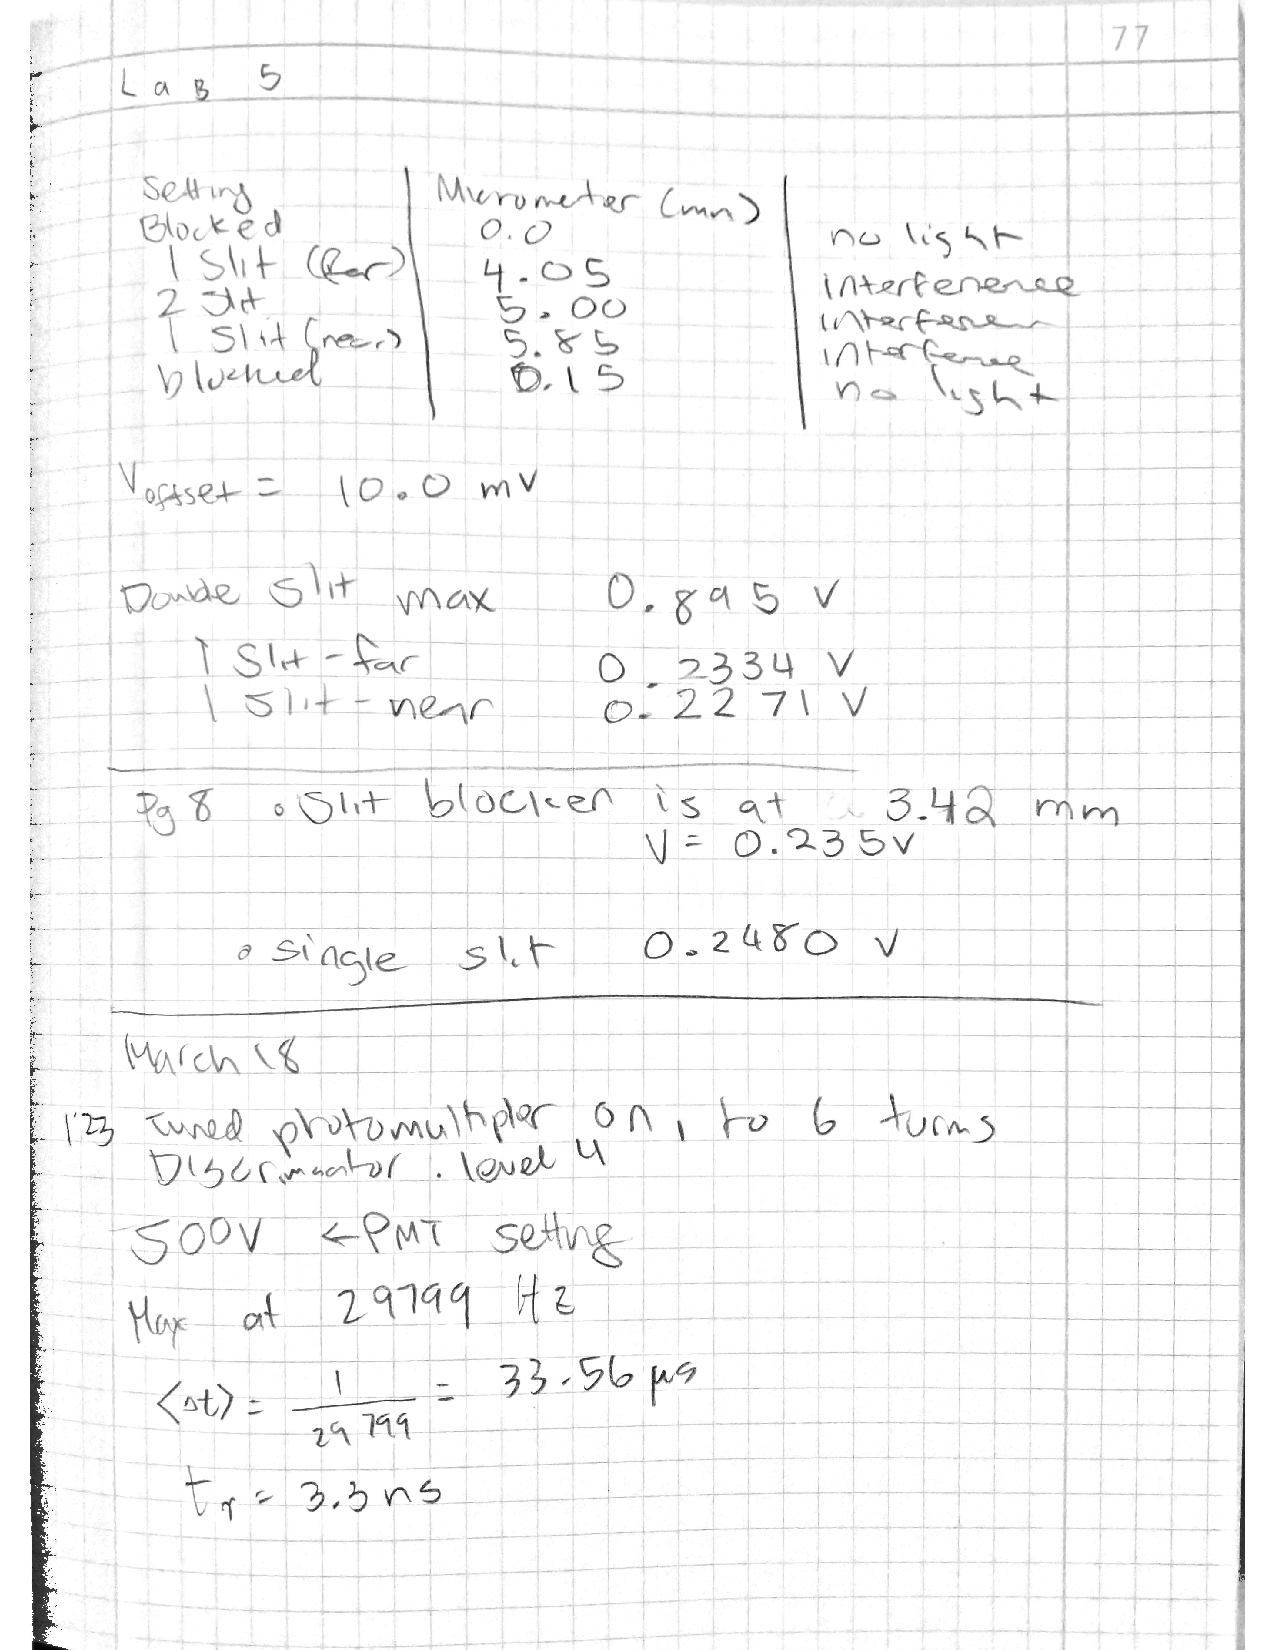
\includegraphics[width=\linewidth]{Scanned_20210401-1937}
	\end{center}
	
\end{document}